% !TEX root = Projektdokumentation.tex
\section{Anhang}
\subsection{Detaillierte Zeitplanung}
\label{app:Zeitplanung}

\tabelleAnhang{ZeitplanungKomplett}

\clearpage
\subsection{Beispiel für ein echtes 1920Schema}
\label{app:RealSchema}
\begin{figure}[htb]
\centering
\includegraphicsKeepAspectRatio{schemaaa.pdf}{0.7}
\caption{Use Case-Diagramm}
\end{figure}

\clearpage


\subsection{Use Case-Diagramm}
\label{app:UseCase}
\begin{figure}[htb]
\centering
\includegraphicsKeepAspectRatio{reneusecase.pdf}{0.7}
\caption{Use Case-Diagramm}
\end{figure}

\subsection{Pflichtenheft (Auszug)}
\label{app:Pflichtenheft}
Es folgt ein Auszug aus dem Lastenheft mit Fokus auf die Anforderungen:

Die Anwendung muss folgende Anforderungen erfüllen: 
\begin{enumerate}[itemsep=0em,partopsep=0em,parsep=0em,topsep=0em]
\item Muss-Kriterien:
	\begin{enumerate}
	\item Datenstrom und Schema müssen frei angegeben werden können.
	\item Das Programm muss den Datenstrom anhand des Schemas zergliedert anzeigen.
	\end{enumerate}
\item Soll-Kriterien:
	\begin{enumerate}
	\item Benutzer sollen ein eingegebenes Schemas speichern können.
	\item Benutzer sollen gespeicherte Schemas laden können.
	\end{enumerate}
\item Kann-Kriterien:
	\begin{enumerate}
    \item Anhand des Transaktionscodes im Datenstrom soll das richtige Schema - falls vorhanden - automatisch ausgewählt werden.
    \item Der Benutzer soll ein Kriterium angeben können, anhand dessen die passenden Datenströme aus der Logdatei ausgewählt werden.
    \item Wenn das Länge-Feld eine Angabe zur Anzahl der Nachkommastellen hat, soll das Programm in der Ergebnis-Anzeige an der richtigen Stelle ein Komma einfügen.

    \item Variablenzeilen sollen ausgeblendet werden können.
        \end{enumerate}
\item Ausschluss-Kriterien:
	\begin{enumerate}
    \item Das Programm soll Schema und Datenstrom nicht auf Korrektheit oder Plausibilität prüfen
(z. B. doppelte Variablennamen, Redefines ohne Vorgänger, ungültige Stufennummern, Bytelänge 0, Char mit Nachkommastellen).
    \end{enumerate}
\end{enumerate}


\subsection{Datenbankmodell}
\label{app:Datenbankmodell}
ER-Modelle kann man auch direkt mit \LaTeX{} zeichnen, siehe \zB \url{http://www.texample.net/tikz/examples/entity-relationship-diagram/}.
\begin{figure}[htb]
\centering
\includegraphicsKeepAspectRatio{database.pdf}{1}
\caption{Datenbankmodell}
\end{figure}
\clearpage

\subsection{Oberflächenentwürfe}
\label{app:Entwuerfe}
\begin{figure}[htb]
\centering
\includegraphicsKeepAspectRatio{MockupModules.pdf}{0.7}
\caption{Liste der Module mit Filtermöglichkeiten}
\end{figure}

\begin{figure}[htb]
\centering
\includegraphicsKeepAspectRatio{MockupModul.pdf}{0.7}
\caption{Anzeige der Übersichtsseite einzelner Module}
\end{figure}

\begin{figure}[htb]
\centering
\includegraphicsKeepAspectRatio{MockupTag.pdf}{0.7}
\caption{Anzeige und Filterung der Module nach Tags}
\end{figure}

\clearpage
\subsection{Screenshots der Anwendung}
\label{Screenshots}
\begin{figure}[htb]
\centering
\includegraphicsKeepAspectRatio{screenshot.pdf}{1}
\caption{Screenshot von 1920Parser (das Ergebnis-Textfeld ist eigentlich etwas breiter)}
\end{figure}
\clearpage

\subsection{Entwicklerdokumentation}
\label{app:Doc}
\begin{center}
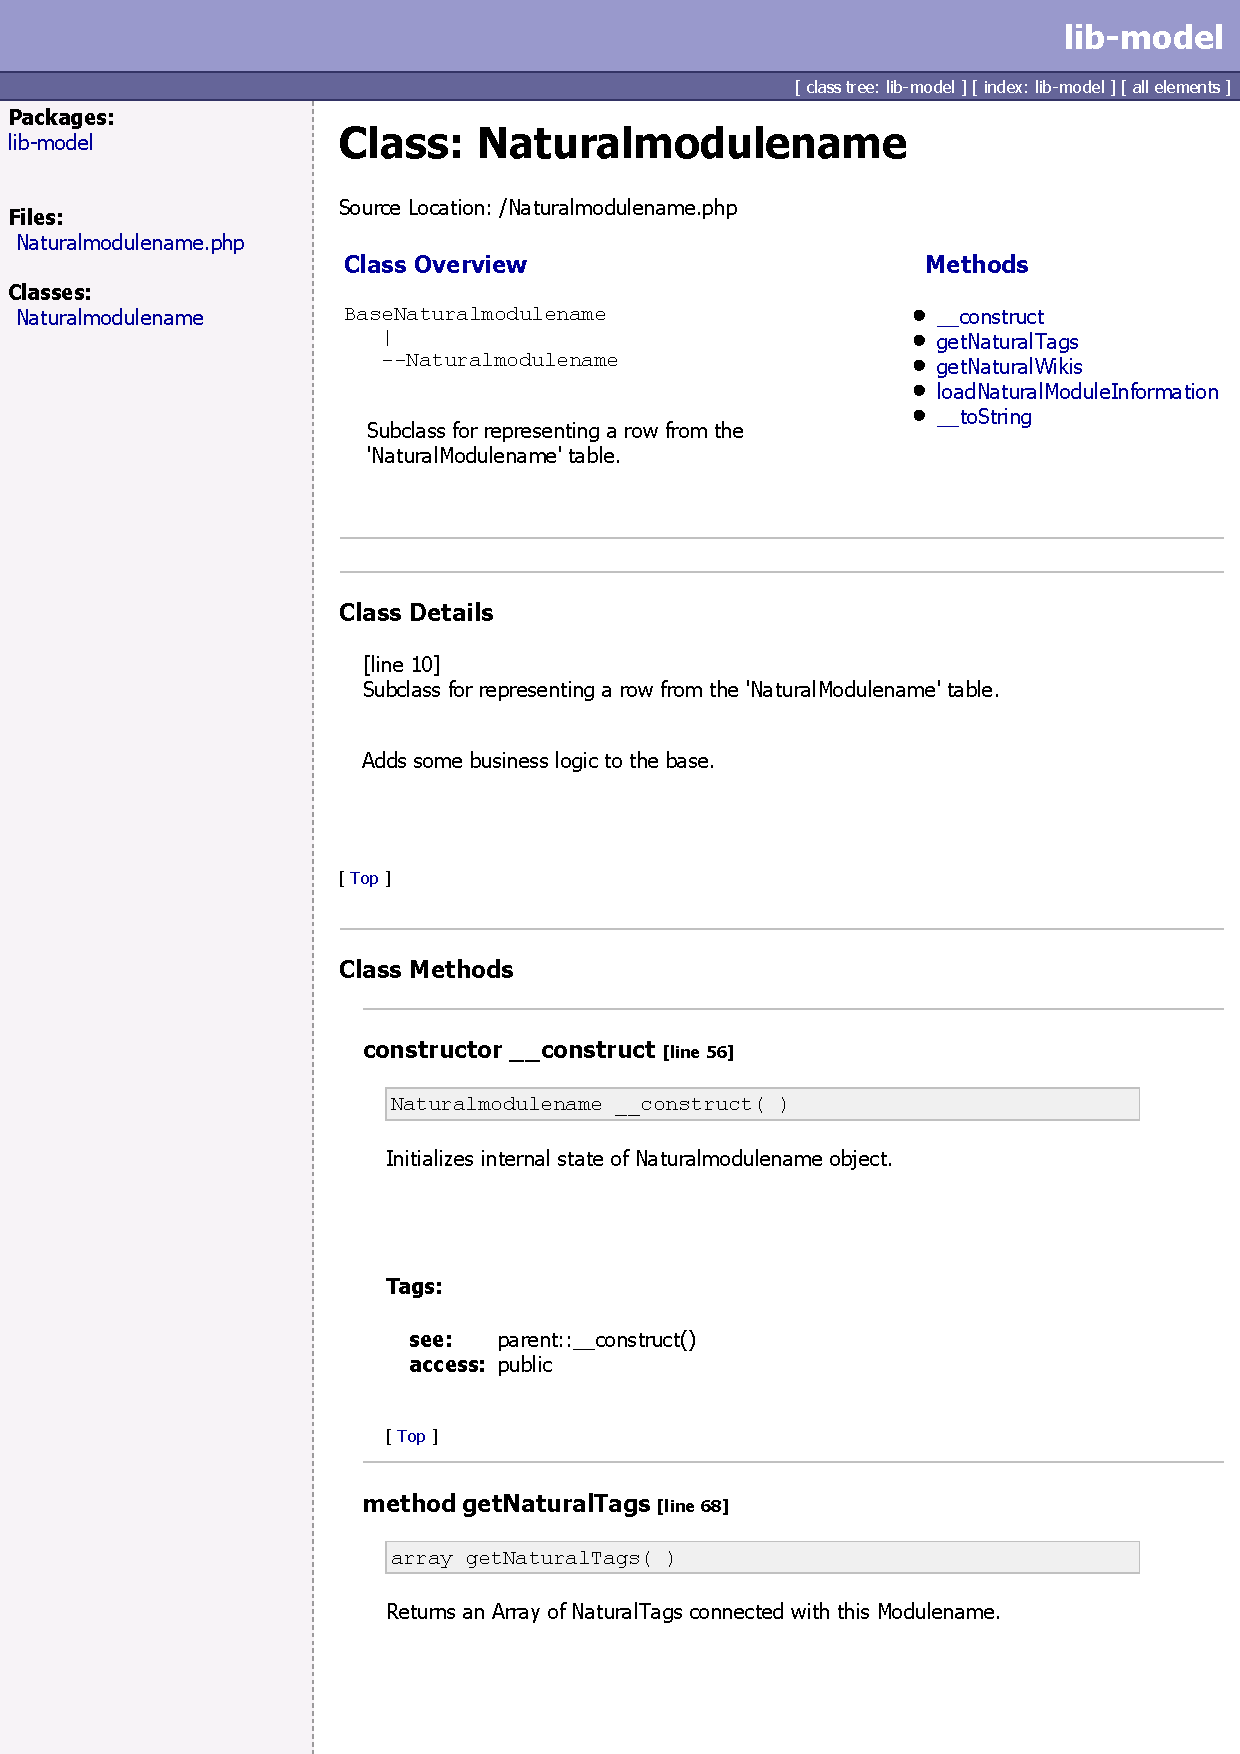
\includegraphics[page=1, width=0.9\textwidth]{doc.pdf}

\includegraphics[page=2, width=0.9\textwidth]{doc.pdf}
\end{center}

\clearpage
\subsection{Testfall und sein Aufruf auf der Konsole}
\label{app:Test}
\lstinputlisting[language=php]{Listings/tests.php}
\clearpage
\begin{figure}[htb]
\centering
\includegraphicsKeepAspectRatio{testcase.jpg}{1}
\caption{Aufruf des Testfalls auf der Konsole}
\end{figure}


\subsection{Klasse: ComparedNaturalModuleInformation}
\label{app:CNMI}
Kommentare und simple Getter/Setter werden nicht angezeigt.
\lstinputlisting[language=php]{Listings/cnmi.php}
\clearpage

\subsection{Klassendiagramm}
\label{app:Klassendiagramm}
Klassendiagramme und weitere \acs{UML}-Diagramme kann man auch direkt mit \LaTeX{} zeichnen, siehe \zB \url{http://metauml.sourceforge.net/old/class-diagram.html}.
\begin{figure}[htb]
\centering
\includegraphicsKeepAspectRatio{Klassendiagramm.pdf}{1}
\caption{Klassendiagramm}
\end{figure}
\clearpage

\subsection{Benutzerdokumentation}
\label{app:BenutzerDoku}
Ausschnitt aus der Benutzerdokumentation:

\begin{table}[htb]
\begin{tabularx}{\textwidth}{cXX}
\rowcolor{heading}\textbf{Symbol} & \textbf{Bedeutung global} & \textbf{Bedeutung einzeln} \\
\includegraphicstotab[]{weather-clear.png} & Alle Module weisen den gleichen Stand auf. & Das Modul ist auf dem gleichen Stand wie das Modul auf der vorherigen Umgebung. \\
\rowcolor{odd}\includegraphicstotab[]{weather-clear-night.png} & Es existieren keine Module (fachlich nicht möglich). & Weder auf der aktuellen noch auf der vorherigen Umgebung sind Module angelegt. Es kann also auch nichts übertragen werden. \\
\includegraphicstotab[]{weather-few-clouds-night.png} & Ein Modul muss durch das Übertragen von der vorherigen Umgebung erstellt werden. & Das Modul der vorherigen Umgebung kann übertragen werden, auf dieser Umgebung ist noch kein Modul vorhanden. \\
\rowcolor{odd}\includegraphicstotab[]{weather-few-clouds.png} & Auf einer vorherigen Umgebung gibt es ein Modul, welches übertragen werden kann, um das nächste zu aktualisieren. & Das Modul der vorherigen Umgebung kann übertragen werden um dieses zu aktualisieren. \\
\includegraphicstotab[]{weather-storm.png} & Ein Modul auf einer Umgebung wurde entgegen des Entwicklungsprozesses gespeichert. & Das aktuelle Modul ist neuer als das Modul auf der vorherigen Umgebung oder die vorherige Umgebung wurde übersprungen. \\
\end{tabularx}
\end{table}


